\chapter{Estado del arte}
En esta sección se van a presentar algunos de los hipervisores más populares utilizados en sistemas embebidos y sus características principales, poniendo más énfasis en los casos de Xen y Jailhouse ya que se tratan de los hipervisores que se han utilizado para el desarrolo del actual TFM. Estos dos últimos resultan de mayor interés debido a que son de código abierto, por lo que aparte de la documentación oficial, a veces un poco escasa en los proyectos de código abierto, exiten repositorios públicos con el código fuente. De esta forma se puede analizar de mejor manera su estructura e incluso modificar partes de su código para adaptarlo a las necesidades del sistema.

\section{OKL4 Hypervisor}
OKL4 Hypervisor es un hipervisor de tipo 1 de los basados en micro-kernel. Fue desarrollado originalmente por OK Labs, la cual forma parte del conglomerado General Dynamics, aprovechando la experiencia en micro-kernels que habían desarrollado gracias al éxito comercial de otro de los productos de OK Labs, el micro-kernel seL4 \cite{seL4}. En su visión, no existían razones para no poder combinar en una única implementación un micro-kernel y un hipervisor. De echo, durante mucho tiempo, el OKL4 se denominó \textit{OKL4 Microvisor}.\\
El objetivo es dar soporte para la virtualización con la mínima sobrecarga del sistema. De esa forma, el modelo propuesto se basa en los siguientes principios \cite{okl4}:
\begin{itemize}
  \item La abstracción de ejecución que presenta el hipervisor a los sistemas operativos guest consta de una o varias CPUs virtuales (vCPU), en las que poder desplegar las tareas requeridas por las aplicaciones de usuario.
  \item En el apartado de virtualización de memoria, el hipervisor proporcioa una MMU virtual (vMMU) con la que se mapea la memoria virtual de los sistemas guest en memoria física del sistema host.
  \item La virtualización de los periféricos, se basa en el mapeo en memoria de registro de dispositivos virtuales y un sistema de interrupciones virtuales (vIRQ).
  \item La comunicacion entre sistemas guest, se muestra como vIRQs (para sincronización) y canales. Los canales se implementan con FIFOs bidireccionales con una tamaño fijo especificado en el espacio de usuario.
\end{itemize}
\begin{figure*}[!htb]
	\centering
	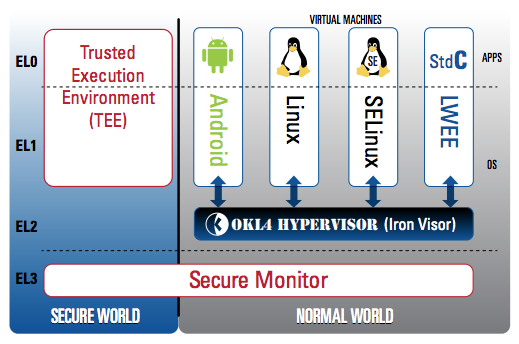
\includegraphics[width=0.65\textwidth]{recursos/OK_L4_Microvisor.png}
	\caption{Ejemplo de arquitectura basada en OKL4 Hypervisor}
	\label{fig:OK_L4_Microvisor}
\end{figure*}
OKL4 Hypervisor proporciona además de soporte de sistemas operativos guest como Linux, VxWorks y Android, un entorno denominado \textit{Lightweight Execution Environments}, que viene a ser un entorno que ofrece rendimentos cercanos a aplicaciones baremetal.




\paragraph{Introducción y Objetivos:}
Justificar la necesidad de desarrollar la tesis en lugar de adquirir o aplicar directamente lo existente a lo largo de la gama de categorías de procesos, productos y servicios de la empresa o institución usuaria de la tesis.
